\begin{figure*}%
	\centering%
	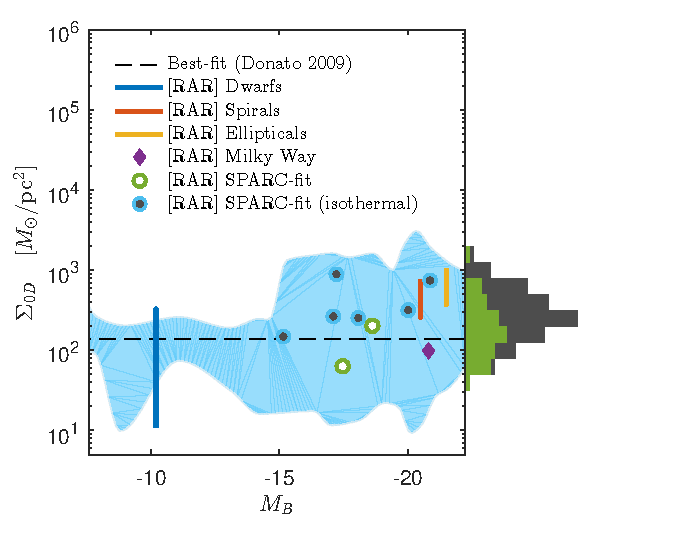
\includegraphics[width=\hsize]{\ROOTPATH/fig.pdf}
	\caption{$\chi^2$ profiles for NGC0055. There is a clear minimum for a total halo mass of $M_s \approx2 \times 10^{10} M_\odot$. Due to the lack of information in the inner halo region the minimum corresponds to a valley in the core mass $10^5 \lesssim M_c \lesssim 10^7$, spanning a range of about 2 orders of magnitude. This uncertainty is also reflected in the cutoff parameter $W_0$. For relatively high values the solutions develop extended isothermal halo tails, which are clearly disfavored here. Solutions with relatively low $W_0$ values, corresponding here to highly cuspy profiles, are ruled out even stronger. Thus, in favor are solutions with mild surface effects.}%
	\label{fig:NGC0055:deep-chi2}%
\end{figure*}